\documentclass[varwidth=true, border=10pt, convert={size=640x}]{standalone}

\usepackage{amsmath}
\usepackage{tikz}
\usetikzlibrary{calc, positioning}
\usepackage{graphicx} % Pour inclure des images
\usepackage{caption}  % Pour les légendes des images
\usepackage{subcaption} % Pour gérer les sous-figures
\usepackage[colorinlistoftodos,prependcaption,textsize=tiny]{todonotes}
\usepackage{pgf}
\usepackage{pgfplots}
\pgfplotsset{compat=1.18}
\usepgfplotslibrary{groupplots}
\usetikzlibrary{arrows.meta} % Needed for 'Circle' arrow tip
\usetikzlibrary{decorations.pathmorphing}

\newlength{\h}
\setlength{\h}{.9cm}

\newcommand{\enc} {\mathsf{AES} }
\newcommand{\drawbc}[5]{%
	% #1: position
	% #2: node name
	% #3: label
	% #4: color
	% #5: size (width and height of the square)

	% Draw square node
	\node[draw, rectangle, minimum width=#5, minimum height=#5,
		inner sep=0pt, align=center, anchor=center, color=#4] (#2) at (#1) {\vphantom{Ay}#3};

	% Triangle perfectly embedded on left side
	\draw[fill=#4, draw=#4]
	($(#2.west) + (0.02, 0.3*#5)$) --  % upper point
	($(#2.west) + (0.02, -0.3*#5)$) -- % lower point
	($(#2.west) + (0.15cm, 0)$) --     % inner tip (fixed width)
	cycle;
}



\newcommand{\BCbloc}[4][]{%
% Dessine le noeud rectangle
\node[#1, draw, rectangle, minimum width=\h, minimum height=\h, anchor=center] (#3) at #2 {#4};
\coordinate (#3/center) at (#3.center);
\coordinate (#3/north) at (#3.north);
\coordinate (#3/east) at (#3.east);
\coordinate (#3/south) at (#3.south);
% Coordonnées du coin inférieur gauche du rectangle pour placer le triangle
\draw[fill=black]
($(#3.north west)!0.15!(#3.north east) - (0, 0.025)$)  -- % Milieu supérieur du côté gauche
($(#3.north east)!0.15!(#3.north west) - (0, 0.025)$) -- % Milieu inférieur du côté gauche
($($(#3.north west)!0.5!(#3.north east)$) - (0, 0.6*0.4*\h)$) -- % Point intérieur (sommet du triangle)
cycle; % Ferme le triangle
}


\begin{document}

\begin{figure}
    \centering
    \resizebox{0.99\textwidth}{!}{
        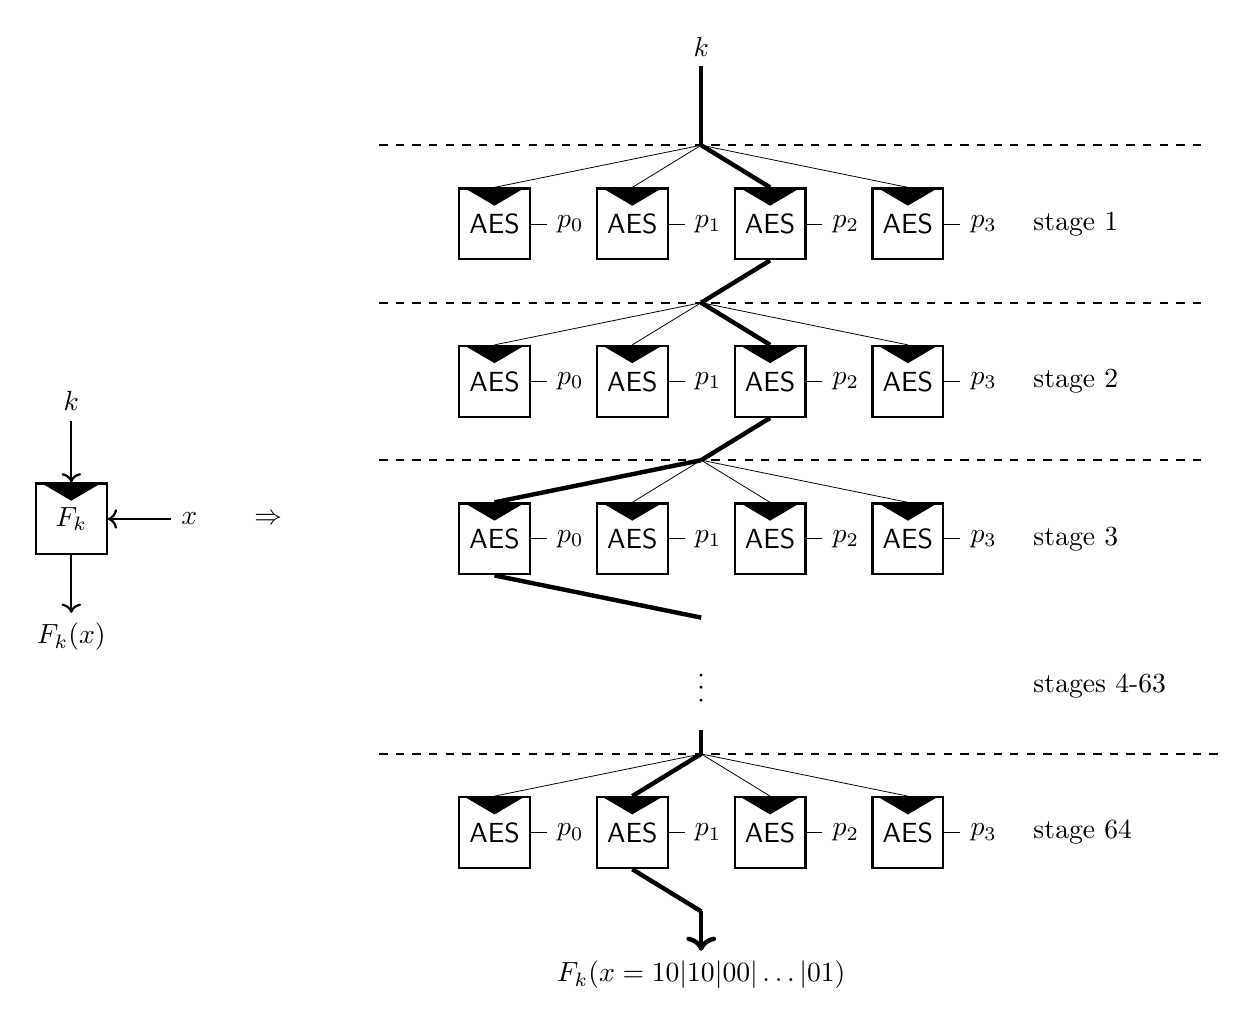
\begin{tikzpicture}[thick, every node/.style={}]
    \def\offPT{0.2cm}
    \def\offDots{0.75cm}
    \def\xoffBC{1.75}
    \def\yoffBC{1}
    \def\Sw{0.1mm}

    \newcommand{\Dots}[1]{
        \node [xshift=-\offDots] at (#1) {$\dots$};
    }

    % 1: id
    % 2: loc anchor i-1
    % 3: layer id
    % 4: bold id
    \newcommand{\Stage}[4]{
        \pgfmathsetmacro{\hOff}{\xoffBC/2}
        \coordinate (#1/e1) at ($#2+(-\hOff,-\yoffBC)$);
        \coordinate (#1/e2) at ($#2+(\hOff,-\yoffBC)$);
        \BCbloc{(#1/e1)}{le1}{$\enc$};
        \BCbloc{(#1/e2)}{le2}{$\enc$};
        \BCbloc{($(#1/e1)+(-\xoffBC,0)$)}{le0}{$\enc$};
        \BCbloc{($(#1/e2)+(\xoffBC,0)$)}{le3}{$\enc$};
        \foreach \xi in {0,...,3}{
            \node [xshift=\offPT, anchor=west] (pt\xi) at (le\xi.east) {$p_{\xi}$};
            \draw [line width=\Sw] (le\xi.east) -- (pt\xi.west); 
            \draw [line width=\Sw] #2 -- (le\xi.north);
        }
        \coordinate (#1/out) at ($#2 + (0,-2*\yoffBC)$);
        \coordinate (#1/in) at #2;

        \foreach \xi in {#4}{
            \draw [ultra thick] (le\xi.north) -- #2;
            \draw [ultra thick] (le\xi.south) -- (#1/out);
        }
        % Node for state indication
        \node [xshift = 1cm, anchor=west] (#1/label) at (le3.east) {stage #3};
        % Draw the dashed line
        \path let \p1=($(le0.west)+(-1,0)$), \p2=($#2+(0,0)$) in coordinate (anch_dash0) at (\x1,\y2);
        \path let \p1=($(#1/label.east)+(1,0)$), \p2=($#2+(0,0)$) in coordinate (anch_dash1) at (\x1,\y2);
        \draw [dashed] (anch_dash0) -- (anch_dash1);
    }

    % The figure in itself
    \node [] (key) at (0, 1.5) {$k$};
    \Stage{st1}{($(key.south)+(0,-\yoffBC)$)}{1}{2};
    \draw [ultra thick] (key.south) -- (st1/in);

    \Stage{st2}{(st1/out)}{2}{2};
    \Stage{st3}{(st2/out)}{3}{0};
    
    % Draw the dots
    \node [anchor=east,yshift=-0.5cm,rotate=90](dots_node) at (st3/out) {$\dots$};
    \path let \p1=(st3/label.west), \p2=(dots_node) in coordinate (anchor_label_other) at (\x1,\y2);
    \node [anchor=west] (lab_other) at (anchor_label_other) {stages 4-63};

    % Draw the last stage
    \Stage{st64}{($(dots_node.west)+(0,-0.5)$)}{64}{1};
    \draw [ultra thick] (st64/in) --++(0,0.3);

    % outputF
    \node [anchor=north, yshift=-0.5cm] (Fx) at (st64/out) {$F_k{(x=10|10|00|\dots|01)}$};
    \draw [ultra thick, ->] (st64/out) -- (Fx.north);

    % Add the top level representation
    \coordinate (locTop) at ($(key) + (-8, -6)$);
    \BCbloc{(locTop)}{topBC}{$F_{k}$};
    \node [yshift=1.5cm ] at (locTop) (ktop) {$k$};
    \node [xshift=1.5cm ] at (locTop) (xtop) {$x$};
    \node [yshift=-1.5cm ] at (locTop) (ytop) {$F_{k}(x)$};
    \draw [->] (ktop.south) -- (topBC/north);
    \draw [->] (xtop.west) -- (topBC/east);
    \draw [->] (topBC/south) -- (ytop.north);

    \node [xshift=1cm] at (xtop) {$\Rightarrow$};


\end{tikzpicture}

    }
    \caption*{Example of instantiation, processing the input per words of 2 bits}
\end{figure}

\end{document}
